\documentclass[a4paper]{article}
\usepackage{geometry}
\usepackage{listings}
\usepackage{color}
\usepackage{graphicx}

\lstset{
frame=tb,
aboveskip=3mm,
belowskip=3mm,
showstringspaces=false,
columns=flexible,
basicstyle={\small\ttfamily},
numbers=none,
numberstyle=\tiny\color{gray},
keywordstyle=\color{blue},
commentstyle=\color{green},
stringstyle=\color{green},
breaklines=true,
breakatwhitespace=true,
tabsize=2
}
\geometry{
a4paper,
total={170mm,257mm},
left=20mm,
top=20mm,
}
\title{Quiz 9: Topic Modeling for Fun and Profit}
\author{Tung Pham}
\date{\today}
\begin{document}
\maketitle
\section{Question 1}
Print all words and their ids from id2word\_wiki where the word starts wtih
"human".

To print the words and ids from id2word\_wiki, I use the following code:
\begin{lstlisting}[language=python]
for word_id, word in id2word_wiki.items():
    if word.startswith("human"):
        print(f"Word: {word}, ID: {word_id}")
\end{lstlisting}

and it produce the following output:

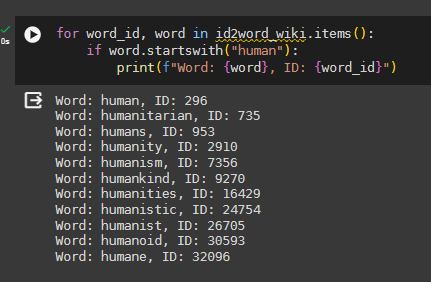
\includegraphics[width=0.8\textwidth]{../images/Q1.png}

\section{Question 2}
Print text transformed into TFIDF space.

To print the text transformed into TFIDF space, I use the following code:
\begin{lstlisting}[language=python]
print([(id2word_wiki[id], tfidf) for id, tfidf in tfidf_model[bow_vector]])
\end{lstlisting}

and below is the output:

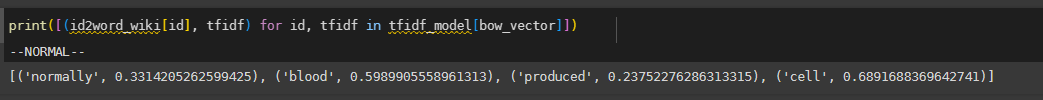
\includegraphics[width=0.8\textwidth]{../images/Q2.png}

\section{Question 3}
Identify the source of difference and change it so they are equivalent.

I change the code section to below, basically only swapping "\_, word" with
"word, \_":

\begin{lstlisting}[language=python]
# select top 50 words for each of the 20 LDA topics
top_words = [[word for word, _ in lda_model.show_topic(topicno, topn=50)] for topicno in range(lda_model.num_topics)]
print(top_words)
\end{lstlisting}

\begin{lstlisting}[language=python]
[
  ['actor', 'singer', 'politician', 'player', 'footballer', 'actress', 'german', 'writer', 'british', 'french', 'president', 'italian', 'director', 'composer', 'canadian', 'musician', 'japanese', 'songwriter', 'prime', 'minister', 'russian', 'poet', 'spanish', 'producer', 'james', 'movie', 'australian', 'king', 'governor', 'killing', 'scottish', 'physicist', 'ii', 'ice', 'robert', 'george', 'journalist', 'charles', 'football', 'david', 'baseball', 'dutch', 'painter', 'general', 'battle', 'begins', 'hockey', 'france', 'television', 'austrian'], 
  ['country', 'countries', 'league', 'government', 'water', 'capital', 'largest', 'population', 'east', 'west', 'century', 'africa', 'land', 'union', 'sea', 'football', 'republic', 'cities', 'language', 'power', 'river', 'million', 'region', 'air', 'empire', 'european', 'live', 'team', 'central', 'important', 'france', 'large', 'international', 'independence', 'western', 'premier', 'climate', 'cup', 'kingdom', 'nations', 'club', 'soviet', 'northern', 'army', 'india', 'al', 'party', 'major', 'mount', 'economy'],
  ['body', 'light', 'earth', 'things', 'example', 'energy', 'water', 'cells', 'species', 'person', 'animals', 'blood', 'usually', 'god', 'transmission', 'small', 'tower', 'mast', 'way', 'uhf', 'word', 'cell', 'means', 'common', 'human', 'theory', 'makes', 'universe', 'living', 'object', 'types', 'form', 'study', 'change', 'large', 'sun', 'live', 'right', 'chemical', 'fish', 'great', 'evolution', 'space', 'temperature', 'important', 'mass', 'plants', 'inside', 'man', 'humans'],
  ['rgb', 'hex', 'color', 'language', 'languages', 'blue', 'web', 'pink', 'red', 'usb', 'esperanto', 'purple', 'green', 'software', 'ff', 'light', 'lake', 'heart', 'crayola', 'bytes', 'disease', 'computers', 'violet', 'cancer', 'linux', 'alphabet', 'yellow', 'words', 'com', 'apple', 'operating', 'magenta', 'data', 'colors', 'chinese', 'free', 'means', 'usually', 'memory', 'drive', 'version', 'os', 'doctors', 'word', 'flash', 'spoken', 'mac', 'writing', 'letters', 'latin'],
  ['president', 'river', 'jpg', 'bush', 'rural', 'file', 'london', 'reagan', 'york', 'germany', 'government', 'party', 'chicago', 'election', 'house', 'capital', 'roman', 'town', 'st', 'washington', 'presidential', 'china', 'bridge', 'famous', 'elected', 'ii', 'george', 'tower', 'urban', 'county', 'great', 'german', 'republican', 'west', 'carter', 'century', 'cities', 'important', 'museum', 'vice', 'virginia', 'office', 'center', 'largest', 'empire', 'dole', 'said', 'bavaria', 'east', 'hugo'],
  ['island', 'church', 'jpg', 'islands', 'sea', 'king', 'europe', 'file', 'country', 'land', 'countries', 'england', 'america', 'large', 'black', 'henry', 'china', 'largest', 'capital', 'built', 'east', 'live', 'mario', 'birds', 'ocean', 'small', 'queen', 'usually', 'great', 'australia', 'house', 'century', 'catholic', 'west', 'kansas', 'population', 'important', 'mountains', 'famous', 'western', 'roman', 'asia', 'building', 'parts', 'px', 'popular', 'cities', 'japan', 'bird', 'sonic'],
  ['music', 'movie', 'band', 'award', 'rock', 'series', 'television', 'movies', 'released', 'film', 'love', 'album', 'played', 'guitar', 'songs', 'doctor', 'song', 'disney', 'awards', 'man', 'popular', 'wrote', 'famous', 'episode', 'star', 'park', 'play', 'children', 'married', 'voice', 'live', 'role', 'father', 'story', 'death', 'studios', 'animation', 'school', 'tv', 'black', 'vocals', 'white', 'heart', 'career', 'nominated', 'lead', 'mother', 'young', 'albums', 'actor'],
  ['game', 'number', 'person', 'example', 'windows', 'player', 'games', 'numbers', 'internet', 'usually', 'way', 'word', 'microsoft', 'school', 'players', 'words', 'gender', 'means', 'ball', 'things', 'sexual', 'play', 'team', 'information', 'version', 'study', 'change', 'autism', 'common', 'children', 'problems', 'help', 'released', 'field', 'written', 'rules', 'nintendo', 'mental', 'include', 'disorder', 'suicide', 'type', 'based', 'types', 'explorer', 'uses', 'computers', 'data', 'social', 'special'],
  ['politician', 'actress', 'actor', 'french', 'german', 'footballer', 'singer', 'british', 'writer', 'italian', 'player', 'president', 'minister', 'king', 'russian', 'ii', 'prime', 'musician', 'canadian', 'scottish', 'composer', 'william', 'japanese', 'france', 'general', 'indian', 'poet', 'governor', 'battle', 'england', 'spanish', 'australian', 'kingdom', 'emperor', 'painter', 'director', 'dutch', 'pope', 'swedish', 'producer', 'paul', 'songwriter', 'george', 'charles', 'author', 'polish', 'leader', 'army', 'henry', 'killed'],
  ['album', 'usually', 'things', 'food', 'bc', 'person', 'band', 'good', 'book', 'god', 'said', 'way', 'money', 'word', 'human', 'countries', 'example', 'century', 'water', 'ancient', 'means', 'making', 'song', 'man', 'fruit', 'milk', 'important', 'released', 'types', 'live', 'books', 'popular', 'love', 'believe', 'right', 'include', 'music', 'death', 'art', 'men', 'think', 'sold', 'metal', 'common', 'body', 'thought', 'gold', 'number', 'public', 'come']
]
\end{lstlisting}
\section{Question 4: Evaluation using Misplaced words.}

To test evaluate this, I myself haven't look at the next cell where it list out
all the replacements and see if I can spotted the word that was misplaced.

The challenge were:
\begin{itemize}
	\item 0 actor singer politician player footballer written german writer british french
	\item 1 country countries league government water temperature largest population east west
	\item 2 body light earth things married energy water cells species person
	\item 3 rgb hex color language languages blue king pink red usb
	\item 4 president light jpg bush rural file london reagan york germany
	\item 5 island church jpg young sea king europe file country land
	\item 6 music movie light award rock series television movies released film
	\item 7 game number person example latin player games numbers internet usually
	\item 8 politician actress actor french german footballer singer british god italian
	\item 9 album usually things food bc person band good president god
\end{itemize}

These are my results:
\begin{itemize}
	\item topic 1: written becuase the other words were about profession or nationality
	\item topic 2: temperature because the other words were about coutnries and nature
	\item topic 3: earth because other things was about human and not nature
	\item topic 4: king because the other words were mostly about cameras and light
	\item topic 5: jpg because the others were about landscape, and regions
	\item topic 6: rock because the words were mostly about films and movies
	\item topic 7: latin because most of the words were about games and numbers
	\item topic 8: god because the other words were about professions and nationality
	\item topic 9: god because most of other words were food and stuff not something that
	      was worship
\end{itemize}

While the actual replacements were:

\begin{lstlisting}[language=python]
[
  (0, ('actress', 'written')),
  (1, ('capital', 'temperature')),
  (2, ('example', 'married')),
  (3, ('web', 'king')),
  (4, ('river', 'light')),
  (5, ('islands', 'young')),
  (6, ('band', 'light')),
  (7, ('windows', 'latin')),
  (8, ('writer', 'god')),
  (9, ('book', 'president'))
]
\end{lstlisting}

Which I got 4 out of 9 right.

I didn't do this for LSI because LSI has almost 200 topics and using this for
all of them is going to take a long time

\section{Question 5: Evaluate using Half and Half}
In order to see the topics assignments of each models, I've modified the code
for intra\_inter like below:

\begin{lstlisting}[language=python]
from collections import defaultdict
import re

def intra_inter(model, test_docs, num_pairs=10000):
    # split each test document into two halves and compute topics for each half
    half = int(len(test_docs)/2)
    part1 = [model[id2word_wiki.doc2bow(tokens[: half])] for tokens in test_docs]

    part2 = [model[id2word_wiki.doc2bow(tokens[half :])] for tokens in test_docs]
    # count the frequency of each topic across all documents
    topic_count1 = defaultdict(int)
    for i, doc_topics in enumerate(part1):
        if len(doc_topics) == 0:
          topic_count2["Unidentified"] +=1
          continue
        top_topic = max(doc_topics, key=lambda x: x[1])[0]
        topic_count1[top_topic] += 1

    topic_count2 = defaultdict(int)
    for i, doc_topics in enumerate(part2):
        if len(doc_topics) == 0:
          topic_count2["Unidentified"] +=1
          continue
        top_topic = max(doc_topics, key=lambda x: x[1])[0]
        topic_count2[top_topic] += 1

    print("Topic count for first part:")
    for topic, count in sorted(topic_count1.items(), key=lambda x: -1 if isinstance(x[0], str) else x[0]):
      print(f"Topic {topic}: {count}")

    print("Topic count for second part:")
    for topic, count in sorted(topic_count2.items(), key=lambda x: -1 if isinstance(x[0], str) else x[0]):
      print(f"Topic {topic}: {count}")
    # print computed similarities (uses cossim)
    print("average cosine similarity between corresponding parts (higher is better):")
    print(np.mean([gensim.matutils.cossim(p1, p2) for p1, p2 in zip(part1, part2)]))

    random_pairs = np.random.randint(0, len(test_docs), size=(num_pairs, 2))
    print("average cosine similarity between 10,000 random parts (lower is better):")
    print(np.mean([gensim.matutils.cossim(part1[i[0]], part2[i[1]]) for i in random_pairs]))
\end{lstlisting}

This code allows me to print out the topics that the model predict each document
to be and then I'll count the occurence that each topic was assigned.

This is the output of running with lda model:

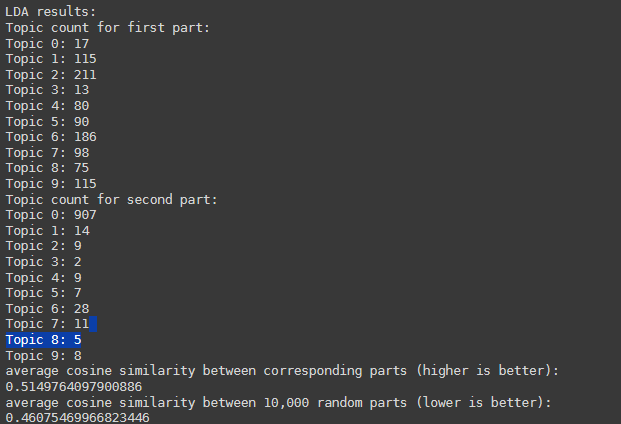
\includegraphics[width=0.8\textwidth]{../images/LDA.png}

We can see that the amount of topics of both are the same.

And this is the output of running with lsi model:

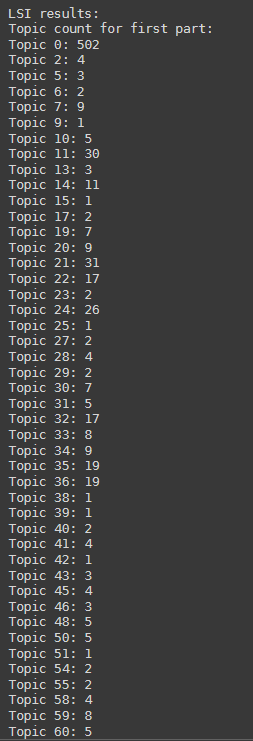
\includegraphics[width=0.8\textwidth]{../images/LSI - 1.png}

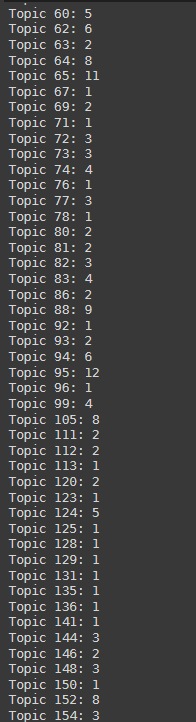
\includegraphics[width=0.8\textwidth]{../images/LSI - 2.png}

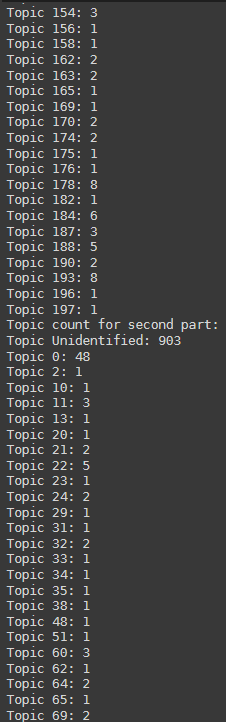
\includegraphics[width=0.8\textwidth]{../images/LSI - 3.png}

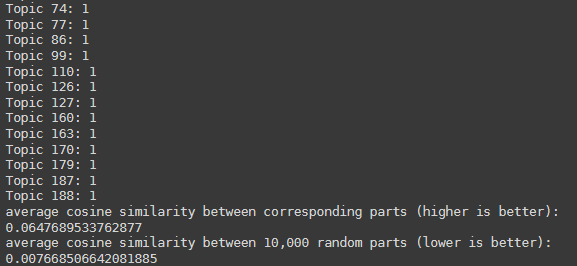
\includegraphics[width=0.8\textwidth]{../images/LSI - 4.png}

However for LSI, we can see that there is a significance difference between the
similar half and the dissimilar half.

Note that because for LSI, there are instances where it can't calculate the
topic of a document and return an empty topic lists, in these instances, we
coutn them as Unidentified.

\section{Question 6: Comparing models}
The intra\_inter metrics for LSI are:
\begin{itemize}
	\item Avg cosine similarity between halves of same doc: 0.0648
	\item Avg cosine similarity between random docs: 0.0082
\end{itemize}

For LDA the numbers are:
\begin{itemize}
	\item Corresponding halves: 0.515
	\item Random halves: 0.462
\end{itemize}

Comparing the value for similar document, we can see that LDA achieves a far
better value compares to LSI. This suggests that LSI failes to capture the
content even within a single document. We can see this from the previous section
where for LSI, we see a lot of Unidentified. Therefore, eventhough LSI produce
lower similarity value for randomized half, it's poor performance against the
similar document is troublesome. In conclusion, I believe that LDA would be a
better choice for this dataset.

\end{document}

